\chapter{非线性差分方程的精确解与$n$阶展开方法}\label{ch04}
尽管线性多项式系数的差分方程并没有被完全解决, 但是它的解从多项式解开始变得越来越一般. 受该方程的解的发展过程的启发, 本文决定求解非线性多项式系数的差分方程的多项式解. 方程的形式为
\begin{equation}
\sum_{k=0}^l{\mbrace{a_k(x)\prod_{i=0}^r{f^{\gamma_{ki}}(x+i)}}}=0.
\label{eq}
\end{equation}
其中, $K$是一个数域, $a_k(x)\in K[x], l>1, \gamma_{ki}\ge 0$. 在本节中, 本文致力于寻找\refeqnn{eq}的所有多项式解. 

受到在微分受到在微分方程求解中被广泛应用的齐次平衡原则的启发, 本文用其求解非线性差分方程的多项式解. 齐次平衡原则通过平衡方程中最高次项的次数来确定解的次数, 只能在一些情况下生效. 本文考虑同时平衡方程中最高$n$项的次数和系数, 提出了$n$阶展开方法来处理齐次平衡原则不能处理的情况, 从而求得\refeqnn{eq}的所有多项式解. 

\section{齐次平衡原则与$n$阶展开方法}
设
\begin{equation}
f(x)=\sum_{k=0}^m{\mu_kx^k},
\label{fm1}
\end{equation}
将其代入\refeqn{eq}, 我们可以求得所有次数不超过$m$的多项式解. 为了求得所有多项式解, 我们需要找到$m$的上界.

将\refeqn{fm1} 代入 \refeqn{eq}后, 方程的左端仍然是一个多项式, 这个多项式的各项次数为
\begin{equation}
D = \mbrace{s_1 m+d_1,s_2 m+d_2,\cdots,s_l m+d_l},
\end{equation}
其中
\begin{equation}
\begin{split}
s_k&=\sum_{i=0}^r{\gamma_{ki}}, \\
d_k&=\deg a_k(x).
\end{split}
\label{eq-sd}
\end{equation}
$D$ 中的每一个次数都是关于 $m$ 的线性表达式, 我们称其为该项的阶数.

方程的左端为零要求整理后的多项式的各项系数为零, 从而要求最高项的系数为零. 因为各个加法项的最高项系数非零, 所以至少有两个不同的最高项进行合并才能使得整理后的多项式最高项系数为零. 从而, 我们有 
\begin{equation}
\left\{
\begin{array}{l}
m\in \mathbb Z_+  ,                                     \\
\exists i\neq j, s_i m+d_i=s_j m+d_j    ,               \\
\forall k \not\in \bbrace{i,j}, s_i m+d_i\ge s_k m+d_k .
\end{array}
\right.
\label{cond}
\end{equation}
上式中的三个约束条件分别被称为: 整数性约束\D 平衡性约束和最大性约束. 

(I) 如果 $s_i \neq s_j$, 我们有 
\begin{equation}
m=\frac{d_j-d_i}{s_i-s_j}.
\end{equation}
如果$m$又同时满足\refeqn{cond}中的其它条件, 则我们称它为第一类平衡点(简称 \BPone{}). 第一类平衡点构成的集合为 
\begin{equation}
M_1=\bbrace{\left. m=\frac{d_j-d_i}{s_i-s_j}\in \mathbb Z_+\right\vert \forall k\not\in \bbrace{i,j}, s_i m+d_i\ge s_k m+d_k}.
\end{equation}

(II) 如果 $s_i = s_j$, 则能够始终满足平衡性约束. 考虑最大性约束, 我们有 
\begin{equation}
\left\{
\begin{split}
m > \frac{d_k-d_i}{s_i-s_k}, & \text{ if } s_i>s_k,  \\
m < \frac{d_k-d_i}{s_i-s_k}, & \text{ if } s_i<s_k.  \\
\end{split}
\right.
\end{equation}
因为\BPone{}的成立条件已经包含上述不等式中取等号的条件, 所以上述不等式不含等号. 求解上述不等式, 可以得到 
\begin{equation}
\underset{s_i>s_k}{\max}{\frac{d_k-d_i}{s_i-s_k}} < m < \underset{s_i<s_k}{\min}{\frac{d_k-d_i}{s_i-s_k}}.
\end{equation}
如果 $s_i m + d_i < \sigma m + \delta$, 则$m$存在上界. 这里, 
\begin{equation}
\begin{split}
\sigma &= \max ~s_k,  \\
\delta &= \underset{s_k=\sigma}{\max}{~d_k}.
\end{split}
\label{eq-max-sd}
\end{equation}

我们可以根$m$是否存在上界, 将剩下的情况细分为两种. 

(II-a) 当 $s_i m + d_i < \sigma m + \delta$时, $m$的取值范围有限. 我们可以得到第二类平衡点(简称 \BPtwo{}). 第二类平衡点构成的集合为
\begin{equation}
M_2=\bbrace{m\in \mathbb Z_+\left|\underset{s_i>s_k}{\max}{\frac{d_k-d_i}{s_i-s_k}} < m < \underset{s_i<s_k}{\min}{\frac{d_k-d_i}{s_i-s_k}}\right.} .
\end{equation}

(II-b) 当 $s_i m + d_i = \sigma m + \delta$ 时, 我们无法基于齐次平衡原则来确定$m$的上界. 因此, 我们提出了一个$n$阶展开方法来解决这个问题.

给定 $n>0$, 我们定义一个$m$次多项式的$n$阶展开多项式为
\begin{equation}
F\sbrace{x,m,u\up n}=\sum_{k=0}^{n-1}{u_k x^{m-k}}+\OO\sbrace{x^{m-n}},
\label{npoly}
\end{equation}
其中 $u\up n=\mbrace{u_0,u_1,\cdots,u_{n-1}}$是系数向量, 而
\begin{equation}
\OO\sbrace{x^n}=\left\{
\begin{array}{cl}
\text{polynomials of degree that no more than } n & n\ge 0, \\
0                                                 & n<0 .
\end{array}
\right.
\end{equation}

对于未知的$m$次多项式$f(x)$, 我们设其最高$n$项的系数为$u\up n=\mbrace{u_0,u_1,\cdots,u_{n-1}}$, 则它可以表示为 
\begin{equation}
f(x)=F\sbrace{x,m,u\up n}.
\end{equation}

对于一个具体的多项式
\begin{equation}
a_k(x)=\sum_{i=0}^{d_k}{a_{k,i} x^{d_k-i}},
\end{equation}
我们设
\begin{equation}
\alpha_{k,i}=\left\{
\begin{array}{cl}
a_{k,i} & i\le \min\{n-1,d_k\}, \\
0       & i >  \min\{n-1,d_k\},
\end{array}
\right.
\end{equation}
则有
\begin{equation}
a_k(x)=F\sbrace{x,d_k,\alpha_k\up n},
\end{equation}
其中, $\alpha_k\up n=\mbrace{\alpha_{k,0},\alpha_{k,1},\cdots,\alpha_{k,n-1}}$.

于是, 在确定了$n$阶展开多项式的基本运算规则之后, 我们就能将\refeqnn{eq}改写为$n$阶展开多项式的形式.

首先, 我们考虑移位操作
\begin{equation}
\Delta^r F\sbrace{x,m,u\up n} = F\sbrace{x+r,m,u\up n} = f(x+r).
\end{equation}
当 $r\neq 0$ 时, 我们有 
\begin{equation}
\begin{split}
\Delta^r F\sbrace{x,m,u\up n} &= \sum_{k=0}^{n-1}{u_k (x+r)^{m-k}}+\OO\sbrace{x^{m-n}} \\
&= \sum_{k=0}^{n-1}{u_k \mbrace{\sum_{j=0}^{m-k}{\binom{m-k}{j}r^kx^{m-k-j}}}}+\OO\sbrace{x^{m-n}} \\
&= \sum_{k=0}^{n-1}{u_k \mbrace{\sum_{m-k-j>m-n}{\binom{m-k}{j}r^kx^{m-k-j}}}}+\OO\sbrace{x^{m-n}} \\
&= \sum_{k+j<n}{u_k {\binom{m-k}{j}r^kx^{m-k-j}}}+\OO\sbrace{x^{m-n}} \\
&=\sum_{p=0}^{n-1}{x^{m-p}\mbrace{\sum_{k=0}^p{u_k\binom{m-k}{p-k}r^{p-k}}}}+\OO\sbrace{x^{m-n}}\\
&=F\sbrace{x,m,v\up n}.
\end{split}
\end{equation}
其中 $v\up n=\mbrace{v_0,v_1,\cdots,v_{n-1}}$, 而
\begin{equation}
v_p=\sum_{k=0}^p{u_k\binom{m-k}{p-k}r^{p-k}}.
\end{equation}

注意到系数$v_p$是关于$m$的多项式, 从而我们不仅可以基于次数来分析$m$的取值, 还能基于系数来分析$m$的取值. 

然后, 我们考虑乘法 
\begin{equation}
\begin{split}
& F\sbrace{x,m,u \up n}\cdot F\sbrace{x,l,v\up n} \\
=& \mbrace{\sum_{k=0}^{n-1}{u_k x^{m-k}}+\OO\sbrace{x^{m-n}}}\mbrace{\sum_{k=0}^{n-1}{v_k x^{l-k}}+\OO\sbrace{x^{l-n}}} \\
=& \mbrace{\sum_{k=0}^{n-1}{u_k x^{m-k}}}\mbrace{\sum_{k=0}^{n-1}{v_k x^{l-k}}}+\OO\sbrace{x^{m+l-n}} \\
=& \sum_{p=0}^{n-1}{x^{m+l-p}\mbrace{\sum_{k=0}^p{u_k v_{p-k}}}}+\OO\sbrace{x^{m+l-n}} \\
=& F\sbrace{x,m+l,w\up n} .
\end{split}
\end{equation}
其中 $w\up n=\mbrace{w_0,w_1,\cdots,w_{n-1}}$, 而
\begin{equation}
w_p=\sum_{k=0}^p{u_k v_{p-k}}.
\end{equation}

在确定了乘法和移位操作之后, 我们就能将\refeqnn{eq}中的每个加法项重写为$n$阶展开多项式的形式, 即
\begin{equation}
\begin{split}
a_k(x)\prod_{i=0}^r{f^{\alpha_{ki}}(x+r)}&=F\sbrace{x,d_k,\alpha_k\up n}\prod_{i=0}^r{\Delta^{\gamma_{ki}}F\sbrace{x,m,u\up n}} \\
&= F\sbrace{x,s_k m+d_k, \omega_k\up n} .
\end{split}
\end{equation}

最后, 我们来考虑更为复杂的
\begin{equation}
F\sbrace{x,s_i m+d_i,u\up n}+F\sbrace{x,s_j m+d_j,v\up n}.
\end{equation}
在一般情况下, 我们不能在$m$未知的情况下比较 $s_i m + d_i$ 和 $s_j m + d_j$ 大小. 但是, 假设
\begin{equation}
s_i m+d_i\ge s_j m+d_j+n, \label{cond_add}
\end{equation}
我们可以有 
\begin{equation}
\begin{split}
&F\sbrace{x,s_i m+d_i,u\up n}+F\sbrace{x,s_j m+d_j,v\up n} \\
=&\left\{
\begin{array}{cl}
    F\sbrace{x,s_i m+d_i,u\up n} & s_i>s_j ,            \\
    F\sbrace{x,s_i m+d_i,w\up n} & s_i=s_j,d_i\ge d_j .
\end{array}
\right.
\end{split}
\end{equation}
其中,
\begin{equation}
w_p=\left\{
\begin{array}{cl}
u_p               & p<d_i-d_j ,   \\
u_p+v_{p-d_i+d_j} & p\ge d_i-d_j.
\end{array}
\right.
\end{equation}

最终, \refeqnn{eq} 能够被重写为
\begin{equation}
F(x,\sigma m + \delta,\Omega\up n)=0. 
\label{eq-np}
\end{equation}
其中 $\Omega\up n=\mbrace{\Omega_0,\cdots,\Omega_{n-1}}$, 而 $\Omega_k$ 则是关于 $m$ 和 $u_k$ 的多项式.

在情况(II-b)的条件下, 根据\refeqn{cond_add}可知, \refeqn{eq-np}中的第 $k$($k=0,1,\cdots$) 个系数有效则要求 
\begin{equation}
\forall s_j<\sigma, \sigma m + \delta - k > s_j m + d_j,
\end{equation}
即
\begin{equation}
m > \underline{m}_k=\underset{s_j<\sigma}{\max}{\frac{d_j-\delta+k}{\sigma-s_j}}.
\end{equation}

现在我们可以来寻找第三类平衡点(简称\BPthree{}). 因为\refeqnn{eq}的左端非零, 因此当$n$足够大时, 必然存在一个$\Omega_k\neq 0$. 设$\Omega_{k_0}$是第一个非零项. 

如果 $\Omega_{k_0}=0$ 关于 $m$ 有非负整数解 $m=m_0$, 则解的次数必然不超过 $m_0$. 同时, $\Omega_{k_0}$ 的有效性又要求 $m>\underline{m}_{k_0}$. 从而, 此类\BPthree{}所构成的集合为 
\begin{equation}
M_3=\bbrace{m\in \mathbb Z_+|\max\sbrace{M_1\cup M_2 \cup \bbrace{\underline{m}_{k_0}}}<m\le m_0}.
\end{equation}

如果 $\Omega_{k_0}=0$ 关于 $m$ 没有非负整数解 $m=m_0$, 就意味着当 $\Omega_{k_0}$有效时, 即$m>\underline{m}_{k_0}$时, 方程没有多项式解. 因此, 方程有多项式解的必要条件是 $m\le \underline{m}_{k_0}$. 从而, 此类\BPthree{}构成的集合为 
\begin{equation}
M_3=\bbrace{m\in \mathbb Z_+|\max\sbrace{M_1\cup M_2}<m\le \underline{m}_{k_0}}.
\end{equation}

最终, 我们可以确定$m$的上界, 即
\begin{equation}
\overline m =\max\sbrace{M_1\cup M_2\cup M_3}.
\end{equation}
将 $f(x)=\sum_{k=0}^{\overline m}{\mu_k x^k}$ 代入 \refeqnn{eq}, 我们就能求得所有多项式解.

\section{方法可视化与典型的例子}
基于\refeqn{cond}中的三个约束条件, 我们确定了解的次数的上界. 因为方程中每一项的次数都是关于$m$的线性表达式, 所以它们能够被看成是平面上的一条直线. 设各项次数为 
\begin{equation}
\lambda_1(m),\cdots,\lambda_l(m). \label{lines}
\end{equation}
其中, $\lambda_k(m)=s_k m+d_k$. 我们的算法等价于在折线
\begin{equation}
\lambda(m)=\max\bbrace{\lambda_1(m),\cdots,\lambda_l(m)} \label{broken_line}
\end{equation}
上寻找两条不同直线的整数交点. 

例如在\reffig{point}中, 有7条直线, 它们分别被记为$\lambda_1,\cdots,\lambda_7$. 这里, 红色表示有多条重复直线, 而黑色表示只有一条直线. 我们用虚线表示\refeqn{lines}中的直线, 用实线表示\refeqn{broken_line}中的折线. 这些直线的交点被标记为$B_1,\cdots,B_8$, 并且我们假设它们都是整点. 
\begin{figure}[H]
\centering
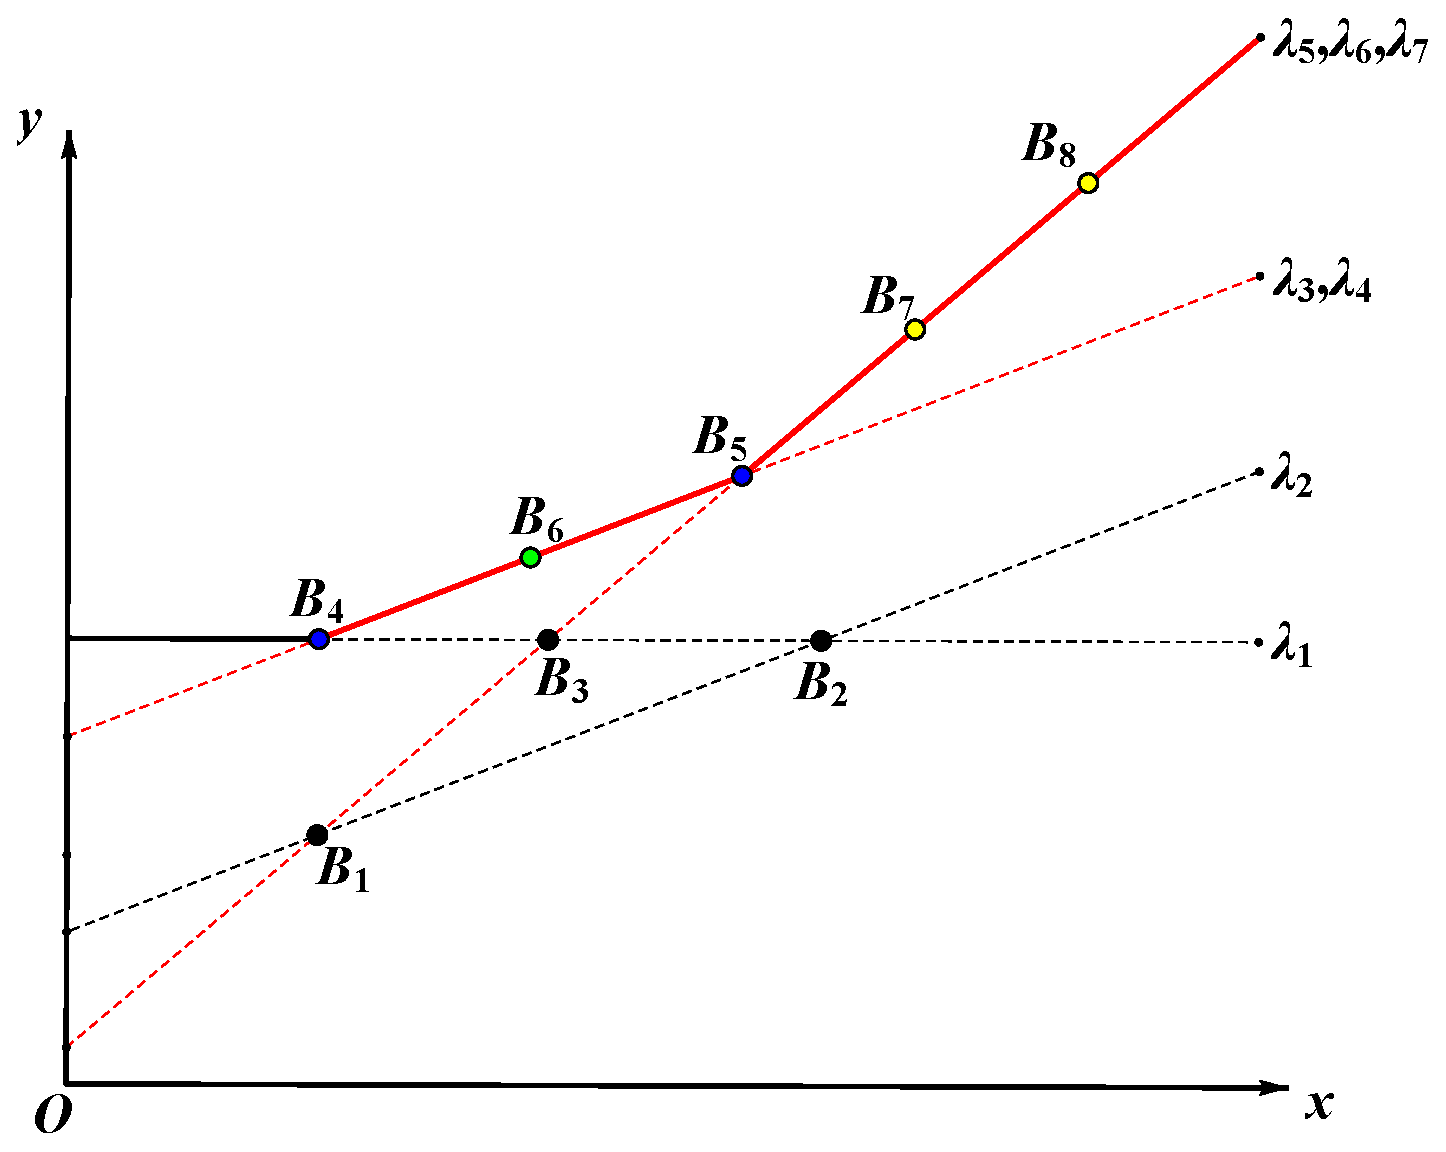
\includegraphics[width=0.6\textwidth]{fig/ps.eps}
\caption{平衡点分类示意图}
\label{point}
\end{figure}
\begin{compactitem}[\textbullet]
\item 尽管$B_1,B_2,B_3$是不同直线的交点, 但是因为它们不满足最大性约束, 所以他们不是平衡点. 
\item 而$B_4,B_5$ 是不同直线的交点且满足最大性约束, 所以它们是第一类平衡点.
\item $B_6$虽然不是不同直线的交点, 但有多条直线穿过它. 又因为它在$B_4$ 和 $B_5$ 之间, 所以它是第二类平衡点.
\item $B_7,B_8$以及它们右侧的更多整点是可能的第三类平衡点\BPthree{}. 因为有多条重复直线穿过它们, 且它们的右侧没有其它直线的交点. 我们可以通过$n$阶展开方法来确定这一类平衡点的上界.
\end{compactitem}

接着, 我们将给出一些具有代表性的例子. 

\begin{example}
(\BPone{})
\begin{equation}
-x^4f(x+3)+(x+1)f(x)^2+8x^6+27x^5+28x^4+2x^3-x-1=0 \label{ep1} .
\end{equation}

我们可以得到其次数列表为$[m+4,2m+1,6]$. 因为没有重复的次数, 所以该方程只有\BPone{}. 从 $m+4=6,2m+1=6$ 和 $m+4=2m+1$ 可以得出 $M_1=\{2,3\}$, 从而$\overline m = 3$. 然后, 将$f(x)=\sum\nolimits_{k=0}^3{\mu_k x^k}$ 代入原方程, 我们可以得到如下方程组:
\begin{equation}
\left\{
\begin{array}{l}
    {\mu_{{0}}}^{2}-1=0,                                                                                                  \\
    {\mu_{{3}}}^{2}-\mu_{{3}}=0,                                                                                            \\
    {\mu_{{0}}}^{2}+2\,\mu_{{0}}\mu_{{1}}-1=0,                                                                                \\
    2\,\mu_{{0}}\mu_{{1}}+2\,\mu_{{0}}\mu_{{2}}+{\mu_{{1}}}^{2}=0,                                                                \\
    2\,\mu_{{2}}\mu_{{3}}+{\mu_{{3}}}^{2}-\mu_{{2}}-9\,\mu_{{3}}+8=0,                                                             \\
    2\,\mu_{{0}}\mu_{{2}}+2\,\mu_{{0}}\mu_{{3}}+{\mu_{{1}}}^{2}+2\,\mu_{{1}}\mu_{{2}}+2=0,                                            \\
    2\,\mu_{{1}}\mu_{{3}}+{\mu_{{2}}}^{2}+2\,\mu_{{2}}\mu_{{3}}-\mu_{{1}}-6\,\mu_{{2}}-27\,\mu_{{3}}+27=0,                              \\
    2\,\mu_{{0}}\mu_{{3}}+2\,\mu_{{1}}\mu_{{2}}+2\,\mu_{{1}}\mu_{{3}}+{\mu_{{2}}}^{2}-\mu_{{0}}-3\,\mu_{{1}}-9\,\mu_{{2}}-27\,\mu_{{3}}+28=0.
\end{array}
\right.
\label{ceqs}
\end{equation}
可以解得, \refeqnn{ceqs}的解为$\{\mu_0=-1,\mu_1=0,\mu_2=0,\mu_3=1\}$. 最终我们得到, \refeqnn{ep1}的多项式解为$f(x)=x^3-1$.
\end{example}

\begin{example}
(\BPtwo{})
\begin{equation}
x^2f(x)f(x+1)f(x+2)+(1-x^9)f(x)+(x^4-x^9)f(x+1)+2x^9f(x+2)-\sum_{k=0}^{10}{c_k x^k}=0, \label{ep2}
\end{equation}
其中$[c_0,\cdots,c_{10}]=[1,1,22,57,85,72,35,9,1,10,6]$. 该方程的次数列表为$[3m+2,m+9,m+9,m+9,10]$. 从$m+9=10$可以得到第一类平衡点$M_1=\{1\}$. 因为$m+9$有两个, 且它关于$m$的系数不是最大的, 所以该方程有\BPtwo{}. 从$\{m+9> 10,m+9> 3m+2\}$可以得出$m< 7/2$. 因此, $\overline m=3$. 然后, 可以解得原方程的多项式解为$f(x)=x^2+x+1$. 显然, 如果不考虑\BPtwo{}, 我们将无法得到该方程的多项式解. 
\end{example}

\begin{example}
(\BPthree{}, 2阶展开)
\begin{equation}
(x+2)f(x)-(x-1)f(x+1)=0. \label{ep3}
\end{equation}
因为该方程的次数列表为$[m+1,m+1]$, 所以它只有\BPthree{}. 基于2阶展开, 即将$f(x)=u_0 x^m + u_1 x^{m-1} + \OO(x^{m-2})$ 代入到原方程中, 可以得到
\begin{equation}
(-u_0 m+3u_0)x^m+\OO(x^{m-1})=0.
\end{equation}
从 $-u_0 m+3u_0=0$ 可以解得 $m=3$. 然后, 基于待定系数法可以可以解得该方程的多项式为 $f(x)=c(x^3-x)$, 其中 $c$ 是任意常数.
\end{example}

\begin{example}
(\BPthree{}, high-order expansion)
\begin{equation}
-2x^5f(x)f(x+2)+x^4f(x)^2+(2x^5-x^4)f(x+1)^2-\sum_{k=0}^{22}{c_k x^k}=0, \label{ep4}
\end{equation}
where $[c_0,\cdots,c_{22}]=$[0, 0, 0, 0, 1, 2046, 10140, 22340, 28095, 20730, 7788, 6120, 30600, 84180, 151164, 199504, 199710, 151380, 85560, 35136, 10035, 1830, 170]. Here, the list of orders is $[2m+5,2m+4,2m+5,22]$. Since $2m+5=22\Rightarrow m=17/2$, this equation only has \BPthree{}. The first nonzero item in the $n$-order expansion is
\begin{equation}
\Omega_3 = 2m^2u_0^2-3mu_0^2-2u_0u_1.
\end{equation}
There is no positive integer solution of $m$. It means that there is no polynomial solution when $2m+5 > 22+3$. In other words, polynomial solution requires $m\le 10$. Thus, $\overline m =10$. Then the solutions of \refeqn{ep4} are $f(x)=\pm (x^{10}-1)$.
\end{example}

\begin{example}
(应用, 2阶展开)

为了计算 
\begin{equation}
    S(x)=\sum_{k=0}^x{k^{10}}
\end{equation}
的闭形式解, 我们可以构造差分方程
\begin{equation}
    S(x)-S(x-1)=x^{10}, S(0)=0. \label{seq}
\end{equation}
该方程的次数列表为$\mbrace{m,m,10}$. 此时, $m=10$ 是 \BPone{}. 因为这里有两个重复的$m$, 所以我们需要考虑\BPthree{}. 该方程的二阶展开为
\begin{equation}
u_0m x^{m-1}+\OO(x^{m-2})=0.   
\end{equation}
因为当$m-1>10$时, $\Omega_1=u_0m$有效, 方程没有多项式解. 所以, 必须有$m\le 11$. 从而, $\overline m=11$. 我们可以得到原方程的多项式解为
\begin{equation}
S(x)=\frac{5}{66}x-\frac{1}{2}x^3+x^5-x^7+\frac{5}{6}x^9+\frac{1}{2}x^{10}+\frac{1}{11}x^{11}.
\end{equation}
从这个例子中也可以看出, 如果不考虑第三类平衡点, 我们也不能得到多项式解. 

另一方面, 因为\refeqnn{seq}是一个线性方程, 它能够被其它方法求解, 例如 \citett{Abramov1989polynomial} 和 \citett{Abramov1995polynomial} 中的方法. 但是, 这个方程在我们的方法中是通过2阶展开进行求解的, 这也说明$n$阶展开方法在我们的算法中是至关重要的.  
\end{example}

\begin{example}
(应用, logistic方程, 也称虫口方程)

因为我们的算法能够找到所有的多项式解, 所以如果我们的算法没有解则表示方程没有多项式解. 考虑著名的logistic 方程\citep{may1976simple}
\begin{equation}
    f(x+1)=r f(x)\sbrace{1-f(x)},
\end{equation}
其中 $r$ 是一个常数. 该方程的阶数列表为 $\mbrace{2m,m,m}$. 因为 $2m\ge m$, 所以该方程只有\BPone{}, 即$2m=m\Rightarrow m=0$. 最终我们可以的得出, 该方程除了$f(x)=0$和$f(x)=(r-1)/r$以外, 没有其它非平凡的多项式解.
\end{example}

\begin{example}
(应用, Riccati方程)

对于 Riccati 方程\citep{bittanti2012riccati}
\begin{equation}
    f(x+1)f(x)+A(x)f(x)+B(x)f(x+1)=C(x), \label{raeq}
\end{equation} 
其中$A(x),B(x)$ 和 $C(x)$ 是多项式系数. 例如取
\begin{equation}
\begin{split}
A(x)&= -\frac{1}{2}\sbrace{x^5+5x^4-40x^2-2}, \\ 
B(x)&= -\frac{1}{2}\sbrace{x^5+10x^3-x-2}, \\ 
C(x)&= -x\sbrace{x+1}\sbrace{48x^4+20x^2-5x-3}.
\end{split}
\end{equation}
则该方程的次数列表为$\mbrace{2m,m+5,m+5,6}$. 对于平衡点的分类讨论如\reftab{tb}所示.

\begin{table}[H]
\centering
\caption{平衡点的分类讨论}\label{tb}
\begin{tabular}{ccc}
\hline
平衡点类型 & 平衡方程 & 平衡点  \\ 
\hline
\BPone{}  & $2m=m+5\ge 6$            & $m=5$             \\ 
\BPone{}  & $2m=6\ge m+5$            & $m\in \varnothing$             \\ 
\BPone{}  & $m+5=6\ge 2m$            & $m=1$             \\ 
\BPtwo{}  & $m+5>\max\bbrace{2m,6}$  & $m\in \bbrace{2,3,4}$ \\
\hline
\end{tabular}
\end{table}
从\reftab{tb}中可以得出$M_1=\bbrace{1,5},M_2=\bbrace{2,3,4}$. 因此, $\overline m=5$. 最终我们可以得到该方程的多项式解为$f(x)=x^5-x$. 

在 Maple 中, 使用 \texttt{rsolve} 求解 \refeqnn{raeq} 会得到
\begin{equation}
\begin{split}
    &f(x)=(f \left( 0 \right) \alpha(x)\,{x}^{5}+f \left( 0 \right) \beta(x)\,{x}^{5}+10\,f \left( 0 \right) \alpha(x)\,{x}^{3}-10\,f \left( 0 \right) \beta(x)\,{x}^{3}+2\,{x}^{5}\\
    &-f \left( 0 \right) \alpha(x)\,x-f \left( 0 \right) \beta(x)\,x-2\,f \left( 0 \right) \alpha(x)+2\,f \left( 0 \right) \beta(x)-2\,x)/(2+2f(0)\alpha(x)) . 
\end{split} \label{rasol_real}
\end{equation}
其中,
\begin{equation}
\begin{split}
&\alpha(x)=\sum_{k_1=0}^{x-1}\mbrace{
    \frac{(-1)^{k_1}p(k_1)}{q(k_1)}\prod_{k_0=0}^{k_1}{
        \frac{q(k_0)}{p(k_0)}
    }
}, \\
&\beta(x)=\sum_{k_1=0}^{x}\mbrace{
    \frac{(-1)^{k_1}p(k_1)}{q(k_1)}\prod_{k_0=0}^{k_1}{
        \frac{q(k_0)}{p(k_0)}
    }
}, \\
&p(x)=x^5+5x^4-20x^2-26x+8, \\
&q(x)=x^5+5x^4+20x^3+10x^2+8x+2. 
\end{split}
\end{equation}
将 $f(0)=0$ 代入\refeqn{rasol_real}, 可以得到 $f(x)=x^5-x$. 这表示该多项式解释在初始条件 $f(0)=0$ 下的解. 此外, 需要注意的是, 使用 \texttt{LRETools[riccati]} 来求解\refeqnn{raeq}将得到错误的解, 这显然是该函数的一个BUG. 
\end{example}

\section{NEM软件包的实现}

The key idea of our algorithm is to find the upper bound of solution degree. It can be summarized as the pseudo-code in Algorithm \ref{findm}. Here, $\mathbb Z_+$ means the set of non-negative integers.

\begin{algorithm}
\newcommand{\kw}[1]{\mathbf{~#1~}}
\newcommand{\Fcn}[1]{\mathtt{#1}}
\renewcommand{\lfrac}[2]{\sbrace{#1}/\sbrace{#2}}
\caption{NEM 核心算法}\label{findm}
\KwIn{Difference equation $eq$ in the form of \refeqn{eq}, expansion order $n$}
\KwOut{Upper bound of solution degree, $-\infty$ means no balance point is found.}
$s,d,\sigma,\delta,l\gets \Fcn{getOrdersOfEqn}(eq)$\;
$m_1,m_2,m_3\gets -\infty$\tcp*[r]{Initial value of three upper bounds.}
$needBP3\gets\kw{false}$\tcp*[r]{Flag variable of whether \BPthree{} is needed.}
\For{$i \kw{from} 1 \kw{to} l$}{\label{for-1-start}
    \For{$j \kw{from} i+1 \kw{to} l$}{
        \uIf(\tcp*[f]{Block of finding \BPone{}.}){$s_i\neq s_j$}{
            $m\gets (d_j-d_i)/(s_i-s_j)$\;
            \If{$m\in \mathbb Z_+ \kw{and} s_im+d_i\ge \max\{s_km+d_k\}$}{
                $m_1\gets \max(m,m_1)$\;
            }
        }\ElseIf{$s_i=\sigma \kw{and} d_i=\delta$}{
            $needBP3\gets \kw{true}$\;
        }\Else(\tcp*[f]{Block of finding \BPtwo{}.}){
            $lb\gets \floor{\underset{s_i>s_k}{\max}{\lfrac{d_k-d_i}{s_i-s_k}}}+1$\;
            $ub\gets \ceil{\underset{s_i<s_k}{\min}{\lfrac{d_k-d_i}{s_i-s_k}}}-1$\;
            \If{$ub\neq +\infty \kw{and} lb\le ub \kw{and} ub\ge 0$}{
                $m_2\gets \max(ub,m_2)$\;
            }
        }
    }
}\label{for-1-end}
\If(\tcp*[f]{Block of finding \BPthree{}.}){$needBP3$}{
    $\Omega\gets \Fcn{getExpansion}(eq,n)$\tcp*[r]{Calculate the $n$-order expansion.}
    \For{$k \kw{from} 0 \kw{to} n-1$}{\label{for-2-start}
        \If{$\Omega_k\neq 0$}{
            $sol\gets \Fcn{solve}(\Omega_k=0,m)$\tcp*[r]{return a set of number.}
            $m_{31}\gets \max(sol \bigcap \mathbb{Z}_+)$\tcp*[r]{$\max(\varnothing)=-\infty$}
            $m_{32}\gets \floor{\underset{s_j<\sigma}{\max}{\lfrac{d_j-\delta+k}{\sigma-s_j}}}$\;
            $m_3\gets \max(m_{31},m_{32})$\;
            \textbf{break}\;
        }
    }\label{for-2-end}
    \If{$m_3=-\infty$}{
        \texttt{warning}(`$n$ need be increased.')\;
    }
}
\Return{$\overline m= \max(m_1,m_2,m_3)$}\;
\end{algorithm}

Firstly, $l$ is the number of items in $eq$, while $s,d,\sigma$ and $\delta$ are calculated by \refeqn{eq-sd} and \refeqn{eq-max-sd}. Then, $m_1,m_2$ and $m_3$ are the upper bound of three kinds of balance points, respectively. The first for-loop between line \ref{for-1-start} and line \ref{for-1-end} is used to calculate $m_1$ and $m_2$. The time complexity of this loop is $\mathcal O(l^3)$. We can determine whether \BPthree{} is needed in the first for-loop, and we using $needBP3$ to record it.

If \BPthree{} is required, the $n$-order expansion of the input equation is calculated by \texttt{getExpansion}. This procedure is implemented by object-oriented programming. The $n$-order expanded polynomial is regarded as an object \texttt{NEPoly}. The major properties of this object are \texttt{p}, \texttt{q} and \texttt{u}. Here, $pm+q$ is the order of this object, \texttt{u} is a coefficient list of length $n$. Then, we override the operations such as add, multiply and shift. After convert undetermined function and coefficient polynomials into \texttt{NEPoly}, the $n$-order expansion can be calculated by Maple automatically. The time complexity of this procedure is $\mathcal O(nl)$.

Then, we will find the first nonzero item of $\Omega$ in the second for-loop between line \ref{for-2-start} and line \ref{for-2-end}. If all items in $\Omega$ are zero, the algorithm will warning user to increase the expansion order $n$. Ignore the complexity of solving polynomial equations, the time complexity of the second for-loop is $\mathcal O(n+l)$.

Finally, the upper bound of solution degree is calculated as the maximum value among $m_1,m_2$ and $m_3$. If no balance point is found, the returned value would be $-\infty$. The time complexity of the whole algorithm is $\mathcal O(l^3+nl+n+l)=\mathcal O(l^3+nl)$.

Based on the key algorithm \texttt{findm}, we implement the whole algorithm of finding all polynomial solutions of \refeqn{eq} in Maple. The invocation interface is
\begin{verbatim}
nlrsolve(eq,fx,{nExpand,inits}).
\end{verbatim}
Here,
\begin{compactitem}[\textbullet]
\item \texttt{eq} is the input equation in the form of \refeqn{eq}.
\item \texttt{fx} is used to specify the unknown function in the form of \texttt{f(x)}. Here, \texttt{f} is the name of unknown function, \texttt{x} is the independent variable of this function.
\item \texttt{nExpand} is optional, it represents the expansion order. The default value is 5.
\item \texttt{inits} is optional, it represents the set of initial conditions. For example, \texttt{\{f(0)=0, f(1)=1\}}.
\end{compactitem}

For example, in order to solve \refeqn{ep4} with the initial condition $\{f(0)=-1\}$ by 4-order expansion, the calling statement is \verb|nlrsolve(eq,f(x),nExpand=4,inits={f(0)=-1})|. Then, we will get the result $\{f(x)=x^{10}-1\}$.

\section{NLREPS软件包的实现与测试}

For difference equations in the form of \refeqn{eq}, our algorithm not only can deduce the considered equation whether has polynomial solutions, but also can find out all polynomial solutions if the considered equation admit them. In order to get enough equations to test our algorithm, we generated 1000 test equations that have polynomial solutions.

The generation of equations is totally based on the random polynomial generation method. Firstly, the original expression $F=\sum_{k=0}^l{\mbrace{a_k(x)\prod_{i=0}^r{f^{\gamma_{ki}}(x+i)}}}$ can be regarded as a multi-variable polynomial with respect to $f(x),\cdots,f(x+r)$ with coefficients $a_k(x)$. Here, $r$ is setting to 3. The degree of this polynomial (i.e., $\max s_k$) is in the range of [3,10]. The maximum degree of coefficient polynomials (i.e., $\max d_k$) is in the range of [1,10]. The number of items in this expression (i.e., $l$) is in the range of [3,500]. Secondly, the maximum degree of the required solution $f^*(x)$ is setting to 10. Finally, substitute $f^*(x)$ into $F$ can get a residual polynomial $g(x)$. Finally, the equation $F-g(x)=0$ has a polynomial solution $f^*(x)$. Based on the generated equations, we will analysis our algorithm from three aspects.

Firstly, the time cost of finding BPs is considered. Since solving polynomial equations is also a time consuming part and is not the duty of our algorithm, we only test the time of finding BPs. The expansion order in the experiment is 5. As we can see in the \reffig{t-findm}, the  increase of time is polynomial, which is consistent with the analysis above.
\begin{figure}[H]
\centering
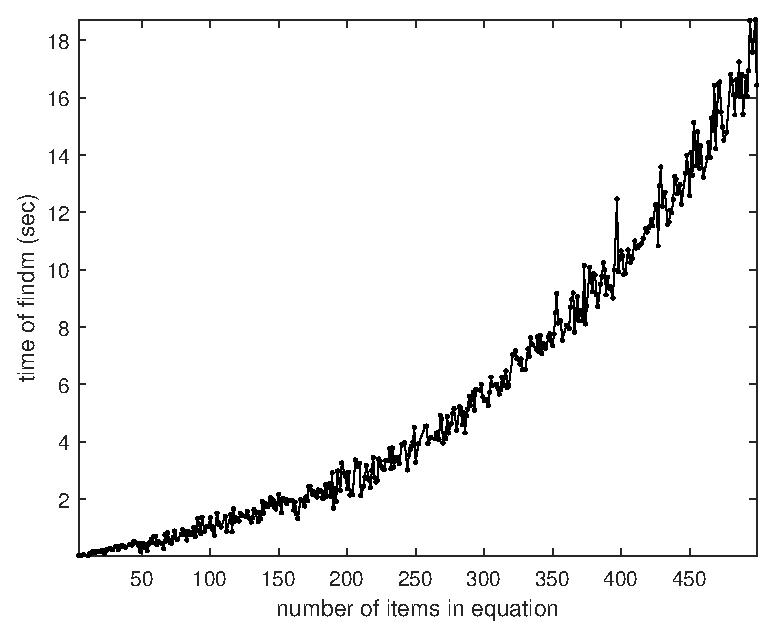
\includegraphics[width=\figwidth]{fig/nlt.eps}
\caption{NLREPS 的时间复杂度}
\label{t-findm}
\end{figure}

Secondly, we are interested in the distribution of BPs. Because there are three types of BPs, and they may occur simultaneously in an equation, we can encode all situations in a binary sequence of length 3. For example, 100 means the equation only has \BPone{}. For the 1000 test equations, the distribution of BPs is shown in \reffig{d-bps}. As we can see, most equations only have \BPone{}. There is no \BPtwo{} in our test. The \BPthree{} only occurs in 4 equations.
\begin{figure}[H]
\centering
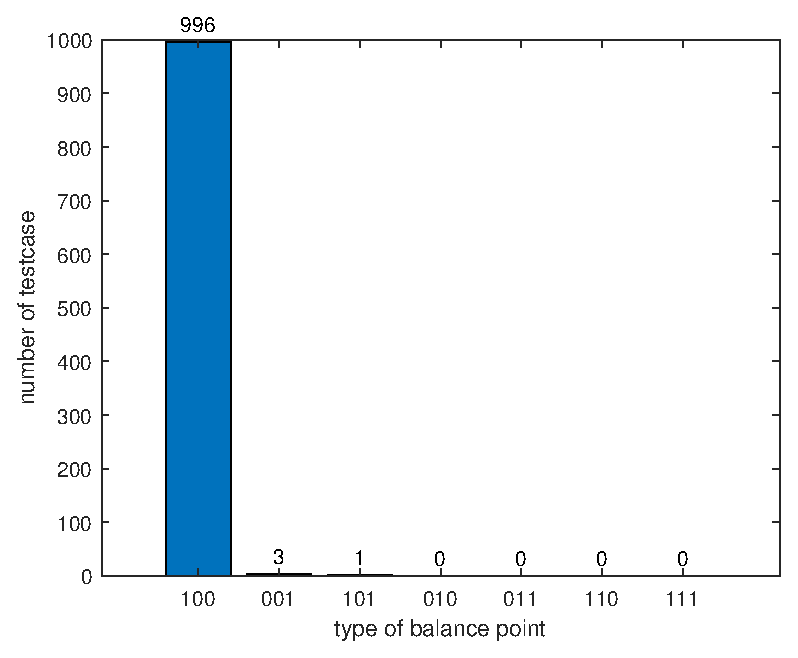
\includegraphics[width=\figwidth]{fig/nbps.eps}
\caption{平衡类型分布}
\label{d-bps}
\end{figure}

Finally, we are interested in the distribution of the least expansion order. Here 1-order expansion means the equation can be solved by homogeneous balance principle. As we can see in \reffig{d-nexp}, only one case need 2-order expansion. This indicates that very few equations require higher order expansion.
\begin{figure}[H]
\centering
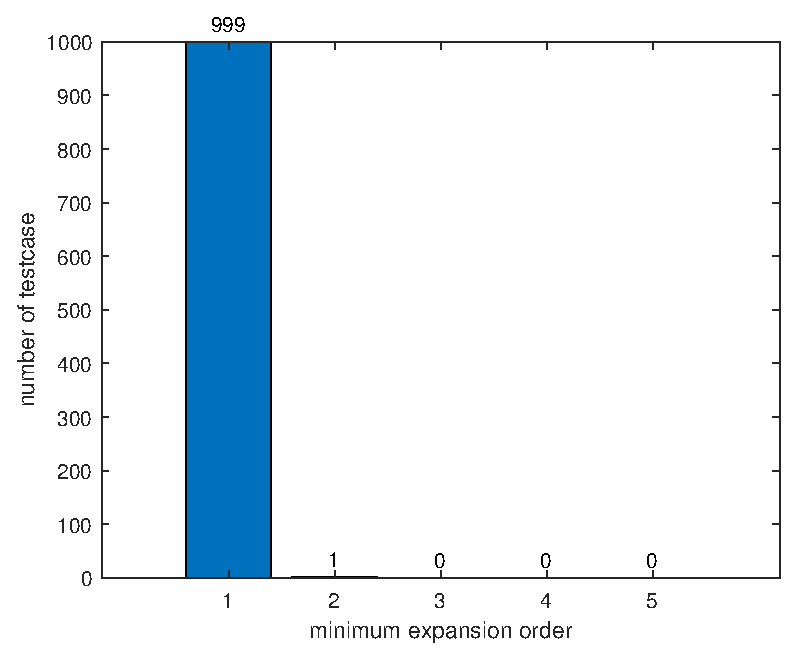
\includegraphics[width=\figwidth]{fig/nexp.eps}
\caption{展开阶数分布}
\label{d-nexp}
\end{figure}

In summary, experiments show that our algorithm has a polynomial time complexity. Furthermore, \BPtwo{} and \BPthree{} are very rare in our test. Since the rarity of \BPthree{}, there are very few cases need $n$-order expansion. So, 5-order expansion is enough for most cases.

\section{关于展开阶数的进一步讨论}

Experiments show that 5-order expansion is enough to solve most problems. In this section, we will analyze it theoretically.

在前文中, the power of $n$-order expanded polynomial is calculated by multiplication. But, it is not feasible when the value of power is undetermined. Now, we are going to infer the rule of power operation. According to the properties of powers,
\begin{equation}
\begin{split}
F\sbrace{x,m,u\up n}^h &= \mbrace{\sum_{k=0}^{n-1}{u_kx^{m-k}}+\OO\sbrace{x^{m-n}}}^h \\
&= \sum_{k=0}^{n-1}{\mbrace{\sum_{b_i}{\frac{h!}{\prod_{i=0}^{n-1}{b_i !}}\prod_{i=0}^{n-1}{u_i^{b_i}}}}x^{hm-k}}+\OO\sbrace{x^{hm-n}} \\
&= F\sbrace{x,hm,v\up n}.
\end{split}
\label{power}
\end{equation}
Here, $\mbrace{b_0,\cdots,b_{n-1}}$ is a non-negative integer solution of
\begin{equation}
\sum_{i=0}^{n-1}{b_i}=h,\sum_{i=0}^{n-1}{ib_i}=k \label{bi}.
\end{equation}
When the solution of \refeqn{bi} is determined, we can get the rule of power.

For $0\le k \le n-1$, let
\begin{equation}
S_k=\bbrace{\mbrace{b_0,\cdots,b_{n-1}}\ge 0 \left| \sum_{i=0}^{n-1}{b_i}=h,\sum_{i=0}^{n-1}{ib_i}=k \right.}.
\end{equation}
It is hard to solve $S_k$ when $h$ is undetermined. The key to our approach is to find a finite set $S^*$ that $\bigcup\nolimits_{k=0}^{n-1}S_k\subset S^*$. Then we can filtrate the elements of $S_k$ from $S^*$ in limited steps.

Since
\begin{equation}
\sum_{i=1}^{n-1}{b_i}\le \sum_{i=1}^{n-1}{i b_i}=\sum_{i=0}^{n-1}{i b_i}=k\le n-1,
\end{equation}
we can get
\begin{equation}
\bigcup\limits_{k=0}^{n-1}S_k\subset S=\bbrace{\mbrace{b_0,\cdots,b_{n-1}}\ge 0 \left| \sum_{i=0}^{n-1}{b_i}=h, \sum_{i=1}^{n-1}{b_i}\le n-1 \right.}.
\end{equation}
Obviously, we have
\begin{equation}
S\subset \overline{S}=\bbrace{\mbrace{b_0,\cdots,b_{n-1}}\left|b_0=h-\sum_{i=1}^{n-1}{b_i},b_i=c_i(i\ge 1),\sum_{i=0}^{n-1}c_i=n-1,c_i\ge 0\right.}.
\end{equation}
The scale of $\overline{S}$ is determined by the number of solutions of
\begin{equation}
\sum_{i=0}^{n-1}c_i=n-1 \label{eqc}.
\end{equation}
Since $n$ is limited, $\overline{S}$ is a finite set.  Hence, $\overline{S}$ is the desired set, i.e., we can assign $S^*=\overline{S}$.

Technically, there are $\binom{2n-2}{n-1}$ non-negative integer solutions of \refeqn{eqc}. Assume  $\mbrace{p_1,\cdots,p_{n-1}}$ is a solution of selecting $n-1$ elements from $\bbrace{1,2,\cdots,2n-2}$, let  $p_0=0,p_n=2n-2$, we can get a related solution of \refeqn{eqc} that $c_k=p_{k+1}-p_k-1$.

Finally, we can calculate $v\up n$ of \refeqn{power} in limited steps.

According to the previous inference, when $n=2$, we can get
\begin{equation}
\mbrace{\Delta^r F\sbrace{x,m,u\up 2}}^h=u_0^h x^{mh}+\sbrace{u_0^hm\cdot hr+u_0^{h-1}u_1\cdot h}x^{mh-1}+\OO\sbrace{x^{mh-2}}
\end{equation}
and
\begin{equation}
\begin{split}
&\mbrace{\Delta^{r_1}F\sbrace{x,m,u\up 2}}^{h_1}\cdot \mbrace{\Delta^{r_2}F\sbrace{x,m,u\up 2}}^{h_2}=u_0^{h_1+h_2} x^{m(h_1+h_2)} \\
+&\sbrace{u_0^{h_1+h_2}m\cdot (h_1r_1+h_2r_2)+u_0^{h_1+h_2-1}u_1\cdot (h_1+h_2)}x^{m(h_1+h_2)-1} \\
+&\OO\sbrace{x^{m(h_1+h_2)-2}}.
\end{split}
\end{equation}
Let
\begin{equation}
G\sbrace{h,q;m,u\up 2}=u_0^h x^{mh}+\sbrace{u_0^hm\cdot q+u_0^{h-1}u_1\cdot h}x^{mh-1}+\OO\sbrace{x^{mh-2}},
\end{equation}
we can get
\begin{equation}
\begin{split}
f(x+r)^h=G\sbrace{h,hr;m,u\up 2}&=\mbrace{\Delta^r F\sbrace{x,m,u\up 2}}^h, \\
G\sbrace{h_1,h_1r_1;m,u\up 2}\cdot G\sbrace{h_2,h_2r_2;m,u\up 2}&=G\sbrace{h_1+h_2,h_1r_1+h_2r_2;m,u\up 2}.
\end{split}
\label{key}
\end{equation}
Hence,
\begin{equation}
\begin{split}
\prod_{i=0}^r{f^{\gamma_{ki}}(x+r)}&=\prod_{i=0}^r{G\sbrace{\gamma_{ki},i\gamma_{ki};m,u\up 2}} \\
&=G\sbrace{\sum_{i=0}^r{\gamma_{ki}},\sum_{i=0}^r{i\gamma_{ki}};m,u\up 2} \\
&=G\sbrace{s_k,t_k;m,u\up 2} \\
&=u_0^{s_k} x^{m{s_k}}+\sbrace{u_0^{s_k}m\cdot {t_k}+u_0^{{s_k}-1}u_1\cdot {s_k}}x^{m{s_k}-1}+\OO\sbrace{x^{m{s_k}-2}} .
\end{split}
\end{equation}
Consequently,
\begin{equation}
\begin{split}
& a_k(x)\prod_{i=0}^r{f^{\gamma_{ki}}(x+r)} = \alpha_{k,0}u_0^{s_k} x^{{s_k}m+d_k} \\
+& \mbrace{\alpha_{k,0}\sbrace{u_0^{s_k}m\cdot {t_k}+u_0^{{s_k}-1}u_1\cdot {s_k}}+\alpha_{k,1}u_0^{s_k}}x^{{s_k}m+d_k-1}+\OO\sbrace{x^{{s_k}m+d_k-2}} .
\end{split}
\end{equation}
When $m\ge\underline{m}_2$, we have
\begin{equation}
\begin{split}
\Omega_0&=\sum_{s_k=\sigma,d_k=\delta}{\alpha_{k,0}u_0^{s_k}}=u_0^\sigma\sum_{s_k=\sigma,d_k=\delta}{\alpha_{k,0}} , \\
\Omega_1&=\sum_{s_k=\sigma,d_k=\delta}\mbrace{\alpha_{k,0}\sbrace{u_0^{s_k}m\cdot {t_k}+u_0^{{s_k}-1}u_1\cdot {s_k}}+\alpha_{k,1}u_0^{s_k}}+\sum_{s_k=\sigma,d_k=\delta-1}{\alpha_{k,0}u_0^{s_k}} \\
&=u_0^\sigma m \sum_{s_k=\sigma,d_k=\delta}{\alpha_{k,0}t_k}+u_0^{\sigma-1}u_1\sigma\sum_{s_k=\sigma,d_k=\delta}{\alpha_{k,0}}+u_0^\sigma\sum_{s_k=\sigma,d_k=\delta-1}{\alpha_{k,0}} .
\end{split}
\end{equation}

The invalidation of 2-order expansion requires $\bbrace{\Omega_0=0,\Omega_1=0}$. It is equivalent to
\begin{equation}
\sum_{s_k=\sigma,d_k=\delta}{\alpha_{k,0}}=0,\sum_{s_k=\sigma,d_k=\delta}{\alpha_{k,0}t_k}=0 .\label{invalid}
\end{equation}
\refeqn{invalid} is a system of linear equations with respect to $\alpha_{k,0} (k=1,\cdots,l)$. Assume that there are $r$ items satisfy $s_k=\sigma$ and $d_k=\delta-1$. When $t_k$ are the same, the dimension of solution space is $r-1$. Otherwise, the dimension of solution space is $r-2$. When $r>2$, \refeqn{invalid} may have non-trivial solutions, the 2-order expansion will be invalid.

For higher order expansion, \refeqn{invalid} is also the necessary condition of invalidation. Generally, coefficients $\alpha_{k,0} (k=1,\cdots,l)$ are in a linear space of dimension $r$. The invalidation of $n$-order expansion restrain coefficients in to a sub-space of dimension $r-\epsilon$. Here, $\epsilon\ge 1$. The probability of these situations is 0.

In a word, the larger expansion order, the less probability of invalidation. So, 5-order expansion is enough for most equations.

\section{小结}

In conclusion, we developed an algorithm that can find all polynomial solutions for nonlinear difference equations in the form of \refeqn{eq}. Both theoretical analysis and experiments show that the algorithm has a polynomial time complexity, which is efficient in practice. For other forms of equations that can be solved by the homogeneous balance principle, the $n$-order expansion method is also useful for the  exceptional cases.
